%\documentclass[11pt,a4paper]{article}
%\usepackage[hyperref]{emnlp2021}
%\usepackage{times}
%\usepackage{latexsym}
%\usepackage{graphicx}
%\usepackage{natbib}
%\usepackage{amsmath}
%\usepackage{amsfonts}
%\usepackage{url}
%\usepackage{multirow}
%\usepackage{booktabs}
%\usepackage{bm}
%\usepackage[linesnumbered, boxed, ruled]{algorithm2e}
%
%\renewcommand\arraystretch{1.2}
%\setlength\parskip{0.1\baselineskip}
%\setlength{\textfloatsep}{0.5cm}
%% This is not strictly necessary, and may be commented out,
%% but it will improve the layout of the manuscript,
%% and will typically save some space.
%\usepackage{microtype}
%\newcommand{\secref}[1]{Section \ref{#1}}
%\newcommand{\figref}[1]{Figure \ref{#1}}
%\newcommand{\eqnref}[1]{Eq. (\ref{#1})}
%\newcommand{\tabref}[1]{Table \ref{#1}}
%\usepackage[hyperref]{emnlp2021}
%\usepackage{times}
%\usepackage{latexsym}
%\usepackage{graphicx}
%\usepackage{natbib}
%\usepackage{amsmath}
%\usepackage{amsfonts}
%\usepackage{url}
%\usepackage{multirow}
%\usepackage{booktabs}
%\usepackage{bm}
%\usepackage[linesnumbered, boxed, ruled]{algorithm2e}
%\usepackage{tikz}
%\usepackage{geometry}
%%\usetikzlibrary{automata,positioning}
%%\geometry{left=2.0cm, right=2.0cm, top=2.5cm, bottom=2.5cm}
\documentclass[11pt,a4paper]{article}
\usepackage{aaai22}  % DO NOT CHANGE THIS                                                                              
\usepackage{times}  % DO NOT CHANGE THIS
\usepackage{helvet}  % DO NOT CHANGE THIS
\usepackage{courier}  % DO NOT CHANGE THIS
\usepackage[hyphens]{url}  % DO NOT CHANGE THIS
\usepackage{graphicx} % DO NOT CHANGE THIS
\urlstyle{rm} % DO NOT CHANGE THIS
\def\UrlFont{\rm}  % DO NOT CHANGE THIS
\usepackage{natbib}  % DO NOT CHANGE THIS AND DO NOT ADD ANY OPTIONS TO IT
\usepackage{caption} % DO NOT CHANGE THIS AND DO NOT ADD ANY OPTIONS TO IT
\DeclareCaptionStyle{ruled}{labelfont=normalfont,labelsep=colon,strut=off} % DO NOT CHANGE THIS
\frenchspacing  % DO NOT CHANGE THIS
\setlength{\pdfpagewidth}{8.5in}  % DO NOT CHANGE THIS
\setlength{\pdfpageheight}{11in}  % DO NOT CHANGE THIS
%\usepackage{algorithm}
%\usepackage{algorithmic}

\usepackage{newfloat}
\usepackage{listings}
\lstset{%
    basicstyle={\footnotesize\ttfamily},% footnotesize acceptable for monospace
    numbers=left,numberstyle=\footnotesize,xleftmargin=2em,% show line numbers, remove this entire line if you don't want the numbers.
    aboveskip=0pt,belowskip=0pt,
    showstringspaces=false,tabsize=2,breaklines=true}

\usepackage{microtype}
\usepackage{natbib}
\usepackage{caption}
\usepackage{helvet}
\usepackage{amsmath}
\usepackage{amsfonts}
\usepackage{tikz}
\usepackage{graphicx}
\usepackage{multirow}
%\usepackage[usenames,dvipsnames]{color}
%\usepackage{color, colortbl}
%\usepackage{subfigure}
\usepackage{url}
\usepackage{bm}
\usepackage{booktabs}
\usepackage{verbatim}
\usepackage[noend]{algpseudocode}
\usepackage{algorithmicx,algorithm}
\usepackage{bbding}
\usepackage{subcaption} 
\setcounter{secnumdepth}{2} %May be changed to 1 or 2 if section numbers are desired.
%\usepackage{aaai22}
%\usepackage{times}
%\usepackage{latexsym}
%\usepackage{graphicx}
%\usepackage{natbib}
%\usepackage{amsmath}
%\usepackage{amsfonts}
%\usepackage{url}
%\usepackage{multirow}
%\usepackage{booktabs}
%\usepackage{bm}
%\usepackage[linesnumbered, boxed, ruled]{algorithm2e}
%\usepackage{bbding}
\newcommand{\crosssymbol}{{ \XSolidBrush} }
%{{\color{red} \XSolidBrush} }
\newcommand{\checksymbol}{{\Checkmark} }
%\renewcommand\arraystretch{1.2}
%\setlength\parskip{0.1\baselineskip}
%\setlength{\textfloatsep}{0.5cm}
% This is not strictly necessary, and may be commented out,
% but it will improve the layout of the manuscript,
% and will typically save some space.
\newtheorem{example}{Example}
\usepackage{microtype}
\newcommand{\secref}[1]{Section \ref{#1}}
\newcommand{\figref}[1]{Figure \ref{#1}}
\newcommand{\eqnref}[1]{Eq. (\ref{#1})}
\newcommand{\tabref}[1]{Table \ref{#1}}
\newcommand{\exref}[1]{Example \ref{#1}}
\newcommand{\cut}[1]{}
%\usepackage{float}
%\usepackage{tikz}
%\usepackage{subfigure}
%\usepackage{graphicx}
%\setlength\footskip{0pt}
%\setlength\headsep{0pt}
%\setlength\topmargin{-50pt}
%\setlength\textheight{800pt}
\title{xxxx}
\author{}
\date{}
\begin{document}
\appendix
\section{Details of Robustness Tests}
\tabref{tab:results} tells more detailed numbers about 
stress test results with different aspects in Figure 4. (Section 3.2)


\begin{table*}[th]
\scriptsize
\centering
\begin{tabular}{ll|c|ccccccc}\hline
\toprule  
\textbf{Dataset}&\textbf{Model}&\textbf{Original} &\textbf{Neg+} & \textbf{Neg-} &\textbf{NER} &\textbf{PR} &\textbf{PI}&\textbf{Voice}&\textbf{All}
                                               \\ 
 \hline
 \multirow{15}{*}{ROC} 
&BT(w/o)&86.58&82.19&59.57&78.18&76.61&90.48&70.22&79.39 \\
&BT+B&86.75&86.14&60.64&86.46&78.66&94.31&70.22&82.41 \\
&BT+C&87.07&80.08&62.77&97.79&88.07&95.93&70.12&83.33 \\
&BT+M&86.48&81.86&79.79&93.09&85&96.75&96.35&88.54 \\
&BT+C+M&86.75&83.36&77.66&97.24&93.2&97.79&97.53&91.40 \\
\cline{2-10}
&XL(w/o)&90.81&88.65&55.32&86.74&50.89&93.5&51.58&73.70 \\
&XL+B&90.43&87.09&60.64&90.88&65.24&94.54&61.24&78.56 \\
&XL+C&89.47&85.7&60.64&99.17&91.61&99.65&64.6&85.60 \\
&XL+M&90.17&87.37&80.85&96.69&74.09&98.84&98.62&89.25 \\
&XL+C+M&90.22&85.53&81.91&99.17&93.38&99.88&98.22&92.88 \\
\cline{2-10}
&RB(w/o)&92.73&85.7&69.15&75.97&67.94&87.34&60.36&76.39 \\
&RB+B&92.46&88.26&62.77&65.19&58.62&77.93&43.79&69.70 \\
&RB+C&91.18&87.76&74.47&99.17&90.49&96.75&75.64&88.00 \\
&RB+M&92.62&86.7&80.85&86.46&76.14&93.73&99.51&88.06 \\
&RB+C+M&91.88&84.97&86.17&99.45&88.35&98.95&99.21&91.79 \\
\hline
\multirow{15}{*}{COPA} 
&BT(w/o)&62&51.42&-&-&55.79&63.47&56.91&55.64 \\
&BT+B&68.6&64.02&-&-&71.95&69.86&72.36&68.64 \\
&BT+C&72.8&69.72&-&-&93.6&77.17&89.43&80.86 \\
&BT+M&70.4&72.15&-&-&83.23&80.37&99.59&81.63 \\
&BT+C+M&72.4&74.8&-&-&87.5&79.91&95.12&82.80 \\
\cline{2-10}
&XL(w/o)&61.4&34.15&-&-&54.88&60.27&79.67&52.61 \\
&XL+B&63.2&88.62&-&-&55.49&64.84&24.8&63.89 \\
&XL+C&67.8&60.16&-&-&83.84&97.26&79.67&76.26 \\
&XL+M&62.2&59.96&-&-&56.4&94.52&100&72.61 \\
&XL+C+M&67.2&82.32&-&-&76.83&98.17&100&87.00 \\
\cline{2-10}
&RB(w/o)&76.4&80.69&-&-&71.04&76.71&67.07&74.94 \\
&RB+B&77&79.67&-&-&82.62&90.87&77.64&81.94 \\
&RB+C&79&79.47&-&-&88.41&97.72&76.83&84.36 \\
&RB+M&72.6&78.46&-&-&86.89&98.63&100&88.17 \\
&RB+C+M&74&87.2&-&-&93.9&100&99.59&93.46 \\
	\hline
\multirow{15}{*}{ARCT} 
&BT(w/o)&63.96&31.65&88.16&80&53.52&60.71&36.78&48.74 \\
&BT+B&68.47&37.04&83.55&60&40.85&48.21&29.31&45.96 \\
&BT+C&68.92&36.7&85.53&100&70.42&76.79&50.57&56.29 \\
&BT+M&67.79&32.32&91.45&80&74.65&82.14&91.95&65.96 \\
&BT+C+M&67.57&36.36&94.08&100&85.92&83.93&91.38&69.27 \\
\cline{2-10} 
&XL(w/o)&75.45&39.39&72.37&20&30.99&51.79&38.51&45.83 \\
&XL+B&79.05&45.12&80.26&40&64.79&57.14&46.55&55.23 \\
&XL+C&74.55&39.73&84.21&60&69.01&82.14&54.6&58.15 \\
&XL+M&74.1&41.75&92.11&40&70.42&80.36&95.4&69.80 \\
&XL+C+M&77.03&45.12&95.39&60&85.92&92.86&95.98&74.44 \\
\cline{2-10} 
&RB(w/o)&78.83&48.82&78.29&60&46.48&42.86&44.83&53.25 \\
&RB+B&81.31&48.82&76.32&60&47.89&58.93&44.25&54.04 \\
&RB+C&77.93&45.12&79.61&60&64.79&69.64&38.51&54.31 \\
&RB+M&77.03&56.57&88.16&40&78.87&85.71&96.55&76.29 \\
&RB+C+M&75&42.42&93.42&60&74.65&87.5&93.68&70.99 \\
	\hline
\multirow{15}{*}{RECLOR} 
&BT(w/o)&45.6&21.87&39.5&-&17.39&42.22&11.45&22.83 \\
&BT+B&48.6&26.93&42.86&-&15.22&42.22&10.69&24.94 \\
&BT+C&47&27.47&56.3&-&63.04&95.56&59.54&49.89 \\
&BT+M&46.8&26.13&53.78&-&56.52&55.56&64.89&46.08 \\
&BT+C+M&43.6&22.13&55.46&-&78.26&77.78&80.92&53.14 \\
\cline{2-10} 
&XL(w/o)&56&25.07&44.54&-&30.43&26.67&13.74&24.93 \\
&XL+B&57&39.2&39.5&-&28.26&42.22&20.61&33.37 \\
&XL+C&54.4&28.53&60.5&-&73.91&91.11&51.15&48.87 \\
&XL+M&53.6&29.33&66.39&-&63.04&68.89&77.86&54.55 \\
&XL+C+M&54.2&33.07&64.71&-&65.22&75.56&77.1&56.47 \\
\cline{2-10} 
&RB(w/o)&50.4&19.47&36.97&-&20.65&20.88&6.46&18.25 \\
&RB+B&51&22.13&39.5&-&28.26&28.89&9.92&22.03 \\
&RB+C&50.4&33.07&60.5&-&89.13&82.22&54.2&51.91 \\
&RB+M&52&31.47&68.91&-&73.91&80&87.79&60.53 \\
&RB+C+M&48.4&26.4&67.23&-&67.39&77.78&81.68&55.77 \\

\bottomrule
\hline
\end{tabular}
\caption{\label{tab:results} Detailed Breakdown of Robustness Tests
on 4 models with or without(w/o) data augmentation. 
+B = augmented with backtranslation,
+C = augmented with crossover, +M = augmented with mutation. 
Robustness Tests includes the following stress tests: 
Neg+=negation-add, Neg-=negation-remove, NER, 
PR=pronoun-replacement, PI=Pronoun-instantiation, Adv=adverbial, Voice, Syn=synonym.}
\end{table*}




\section{Details of Choice-only test}
In~\tabref{tab:only-test}, we show specific numbers for Figure 5 which describe 
the choice-only results. (Section 3.3)
\begin{table}[th]
\centering
\scriptsize
\begin{tabular}{c|rrrr}
\toprule
\textbf{Model} & \textbf{ROC} & \textbf{COPA} & \textbf{ARCT} & \textbf{RECLOR} \\ \midrule
BT (w/o)&54.62&51.4&61.94&42.8 \\ \hline
BT+B&58.26&50.8&64.41&39.2  \\ \hline
BT+C&51.2&48.2&55.63&30.8  \\ \hline
BT+M&51.79&48.8&55.18&38   \\ \hline
BT+C+M&43.56&49.4&52.03&33.8  \\ \midrule
XL (w/o)&71.14&57&65.99&42.2 \\ \hline
XL+B&73.17&60&66.89&41.4  \\ \hline
XL+C&65.63&55&55.86&34.2  \\ \hline
XL+M&71.94&57.8&66.22&42  \\ \hline
XL+C+M&66.22&58.4&62.84&35  \\ \midrule
RB (w/o)&73.97&59.4&67.79&30.2 \\ \hline
RB+B&74.77&61.4&69.37&42.2  \\ \hline
RB+C&73.06&58.4&68.47&34.6  \\ \hline
RB+M&70.34&56&61.49&40      \\ \hline
RB+C+M&71.3&54.8&67.79&32.2  \\ 
\bottomrule
\end{tabular}
\caption{Choice-only test for transformer-based models on 4 datasets. All numbers are percentages (\%)}
%\KZ{I assume this is the ending-only test? But isn't smaller the better
%for ending-only tests?}}
\label{tab:only-test}
\end{table}

\section{Extra Cases}
We have shown an example in Section 3.4 for the case study. In this section of the appendix, we 
provide extra 3 cases for further illustrating that \textit{crossover} and \textit{mutation} 
encourage models to build contextual reasoning  
by attending to relevant concepts in the premise. 
%can better enourage transformer-based models to pay attention to premise and the relationship 
%between premise and choices. 

\begin{example}\label{ex:roc}
An MCQ from ROC:\\ \\
\noindent
\textbf{Premise:} Sarah was home alone. She wanted to stay busy. She turned on the TV. 
She found a reality show to watch.  \\
\textbf{Choice 1:} Sarah then happily watched the show.  \checksymbol  \\
\textbf{Choice 2:} Sarah could not find anything to watch. \crosssymbol
\end{example}

In \exref{ex:roc}, we explore BERT-based models by 
analyzing their attention maps on this question in~\figref{fig:roc_bert}.  
There is no 
positive attention value in front of the fourth sentence, 
so we intercept it from where it is worth. 
BERT trained on the original training set fails 
to pick up the right choice likely due to there being 
virtually no attention connection between words in 
the choice and words in the premise.
After training with \textit{crossover} data augmentation, 
the model learns  
to pay attention to premise and the relationship 
between premise and choices. 
i.e., ``show'' in this example. The rationale behind 
such a change of attention pattern is that, 
in an MCQ created by \textit{crossover} operation (\figref{fig:roc_c}), \textit{mutation}(\figref{fig:roc_m}), 
and the combination of them (\figref{fig:roc_cm})
the model needs to combine the information 
in the premise to effectively 
distinguish the true ``right'' choice from the wrong one. 
However, the light and sparse attention color blocks on the attention map for back-translation 
in \figref{fig:roc_b} indicate back-translation 
can not help BERT connect the choice and premise very well in this question.

\begin{figure}[th!]
\centering
\begin{subfigure}[b]{0.20\textwidth}
\centering
\framebox{\includegraphics[width=\columnwidth]{figure/roc_o.eps}}
\caption{BT(w/o)}
\label{fig:roc_o}
\end{subfigure}
\hfill
\newpage
\begin{subfigure}[b]{0.20\textwidth}
\centering
\framebox{\includegraphics[width=\columnwidth]{figure/roc_b.eps}}
\caption{BT+B}
\label{fig:roc_b}
\end{subfigure}
\hfill
\begin{subfigure}[b]{0.20\textwidth}
\centering
\framebox{\includegraphics[width=\columnwidth]{figure/roc_c.eps}}
\caption{BT+C}
\label{fig:roc_c}
\end{subfigure}
\hfill
\newpage
\begin{subfigure}[b]{0.20\textwidth}
\centering
\framebox{\includegraphics[width=\columnwidth]{figure/roc_m.eps}}
\caption{BT+M}
\label{fig:roc_m}
\end{subfigure}
\hfill
\begin{subfigure}[b]{0.20\textwidth}
\centering
\framebox{\includegraphics[width=\columnwidth]{figure/roc_cm.eps}}
\caption{BT+C+M}
\label{fig:roc_cm}
\end{subfigure}
\caption{Attention map on a ROC example for BERT-based models.}
%\KZ{Caption is wrong! most graphs are fine. 
%But ReCLOR (RB) is a bit strange. 
%Why is BT line exactly the same as the BT+C? And why is BT+B so bad?}}
\label{fig:roc_bert}
\end{figure}


\begin{example}\label{ex:copa2}
An MCQ from COPA:\\ \\
\noindent
\textbf{Premise:} I was furious.\\
\textbf{Choice 1:} I slammed the door upon leaving the house.  \checksymbol \\
\textbf{Choice 2:} I checked the mailbox upon leaving the house. \crosssymbol
\end{example}

\begin{figure}[th!]
\centering
\begin{subfigure}[b]{0.20\textwidth}
\centering
\framebox{\includegraphics[width=\columnwidth]{figure/copa2_o.eps}}
\caption{XL(w/o)}
\label{fig:copa2_o}
\end{subfigure}
\hfill
\newpage
\begin{subfigure}[b]{0.20\textwidth}
\centering
\framebox{\includegraphics[width=\columnwidth]{figure/copa2_b.eps}}
\caption{XL+B}
\label{fig:copa2_b}
\end{subfigure}
\hfill
\begin{subfigure}[b]{0.20\textwidth}
\centering
\framebox{\includegraphics[width=\columnwidth]{figure/copa2_c.eps}}
\caption{XL+C}
\label{fig:copa2_c}
\end{subfigure}
\hfill
\newpage
\begin{subfigure}[b]{0.20\textwidth}
\centering
\framebox{\includegraphics[width=\columnwidth]{figure/copa2_m.eps}}
\caption{XL+M}
\label{fig:copa2_m}
\end{subfigure}
\hfill
\begin{subfigure}[b]{0.20\textwidth}
\centering
\framebox{\includegraphics[width=\columnwidth]{figure/copa2_cm.eps}}
\caption{XL+C+M}
\label{fig:copa2_cm}
\end{subfigure}
\caption{Attention map on a COPA example for XLNet-based models.}
%\KZ{Caption is wrong! most graphs are fine. 
%But ReCLOR (RB) is a bit strange. 
%Why is BT line exactly the same as the BT+C? And why is BT+B so bad?}}
\label{fig:copa2_bert}
\end{figure}

In human cognition, the word ``furious'' in premise and ``slammed'' in the right choice 
have a strong causal relationship in~\exref{ex:copa2}. 
However, from the attention map of the vanilla XLNet model in \figref{fig:copa2_bert}, 
it is difficult to observe that they are related. 
In \figref{fig:copa2_bert}, we also observe that 
the ability of XLNet to use relationships has been strengthened by adding augmented data with all 
methods we mentioned. Back-translation is worse than the other methods with lighter color blocks.

\begin{example}\label{ex:arct1}
An MCQ from ARCT:\\ \\
\noindent
\textbf{Premise:} I would be happy to support free community college so those who can't afford it can get educated. College should be free.\\
\textbf{Choice 1:} I would be happy to pay tuition for everyone , even some rich kids.  \checksymbol \\
\textbf{Choice 2:} I would not be happy to pay for some rich kids tuition at the same time. \crosssymbol
\end{example}

\begin{figure}[th!]
\centering
\begin{subfigure}[b]{0.20\textwidth}
\centering
\framebox{\includegraphics[width=\columnwidth]{figure/arct1_o.eps}}
\caption{BT(w/o)}
\label{fig:arct1_o}
\end{subfigure}
\hfill
\newpage
\begin{subfigure}[b]{0.20\textwidth}
\centering
\framebox{\includegraphics[width=\columnwidth]{figure/arct1_b.eps}}
\caption{BT+B}
\label{fig:arct1_b}
\end{subfigure}
\hfill
\begin{subfigure}[b]{0.20\textwidth}
\centering
\framebox{\includegraphics[width=\columnwidth]{figure/arct1_c.eps}}
\caption{BT+C}
\label{fig:arct1_c}
\end{subfigure}
\hfill
\newpage
\begin{subfigure}[b]{0.20\textwidth}
\centering
\framebox{\includegraphics[width=\columnwidth]{figure/arct1_m.eps}}
\caption{BT+M}
\label{fig:arct1_m}
\end{subfigure}
\hfill
\begin{subfigure}[b]{0.20\textwidth}
\centering
\framebox{\includegraphics[width=\columnwidth]{figure/arct1_cm.eps}}
\caption{BT+C+M}
\label{fig:arct1_cm}
\end{subfigure}
\caption{Attention map on an ARCT example for BERT-based models.}
%\KZ{Caption is wrong! most graphs are fine. 
%But ReCLOR (RB) is a bit strange. 
%Why is BT line exactly the same as the BT+C? And why is BT+B so bad?}}
\label{fig:arct1_bert}
\end{figure}

In~\exref{ex:arct1}, the claim and reason are ``College should be free'' and 
``I would be happy to support ... who can't afford it can get educated'' separately. 
The word ``free'' is very important for the claim. 
It should be very related to the information in the correct warrant, 
such as ``tuition'' or ``pay'' from the knowledge of commonsense reasoning. 
Unfortunately, ``free'' has little relationship with the warrant in~\figref{fig:arct1_o}
through the vanilla BERT model. 
Consistent with our previous conclusion, 
the improvement effect of \textit{crossover} and \textit{mutation} 
is more obvious than back-translation. 
Besides, we also observe that the performance of data augmentation methods 
is not as obvious as the first two examples. 
One reason may be that analyzing with this white-box method is not completely reliable. 
The other may be that the ability of these data augmentation methods to reduce short circuits 
and to improve the stability of the model is limited. 
We will continue to study the reason in the future.





\end{document}
